\section{Results}
Selected preprocessing / serving / mapping approaches
Survey results
The map application

\subsection{Data preprocessing}

\ref{tab:preprocessing methods}

\begin{table}[H]
	\caption{
		The assessment of the preprocessing methods.
		The methods applying the highest levels of geometrical simplification
		resulted in the largest increases in map responsiveness,
		but also resulted in significant information loss when mapping the data.
	}
	\label{tab:preprocessing methods}
	\centering
	\begin{tabular}{ | L{0.25\textwidth} | L{0.33\textwidth} | L{0.33\textwidth} | }
		\hline
		\textbf{Method, type of optimization}
		& \textbf{Increase in responsiveness of the map}
		& \textbf{Loss of information on the map}
		\\
		\hline
		\hline
		Aggregation into isochrone polygons (15-minute interval),
		\textit{Reducing geometrical complexity and file sizes}.
		& Large: The isochronal approach is what makes the real-time interaction possible.
		& Large: 15-minute isochrone polygons allow for quick overview
		but make detailed assessment impossible.
		\\
		\hline
		Limiting the maximum travel time (60 minutes),
		\textit{Reducing geometrical complexity and file sizes}.
		& Noticeable on all travel modes, as the largest isochrone polygons are more costly to render.
		The more data was discarded, the larger the increase:
		most increase observed when mapping the slowest travel modes.
		& Depends on travel mode:
		For walking a limit of 60 minutes means that, on average,
		the isochrones cover 3\% of the total area of the dataset.
		For cycling 30\%, for public transit 27\%, for car 98\%.
		For a given grid cell the averaged coverage of all modes is 40\%.
		\\
		\hline
		Limiting coordinate precision,
		\textit{Reducing file sizes}.
		& Potentially noticeable with limited download speeds:
		Reducing the precision of geometries reduced file sizes by 50\% on average,
		thus enabling faster data transfer.
		No visible effect on responsiveness was observed in this study.
		& None: The decreased precision is in no way visible.
		\\
		\hline
		Minimizing files by simplifying GeoJSON structure and compressing using gzip,
		\textit{Reducing file sizes}.
		& Potentially noticeable with limited download speeds:
		This reduces file sizes by 60\% on average,  % TODO
		thus enabling faster data transfer.
		No visible effect on responsiveness was observed in this study.
		& None: These approaches do not affect the content of the data.
		\\
		\hline
	\end{tabular}
\end{table}


\subsection{Backend solution}

\subsection{Mapping libraries}

\begin{table}[H]
	\caption{Comparison of mapping libraries}
	\label{tab:map library comparison}
	\centering
	\begin{tabular}{ | L{0.1\textwidth} | L{0.25\textwidth} | L{0.25\textwidth} | L{0.25\textwidth} | }
		\hline
		Library
		& Quality of visualization
		& Rendering performance
		& Integration with React
		\\ 
		\hline
		\hline
		Deck.gl
		& Inconsistent rendering of complex polygons, vector tiles supported
		& GPU accelerated (WebGL), most performant of the tested libraries
		& Designed from ground up to work with React
		\\
		\hline
		Leaflet
		& Correct rendering of polygons, Vector tiles possible through plugins
		& No GPU acceleration, least performant of the tested libraries
		& Integration possible with a 3rd party wrapper
		\\
		\hline
		Maplibre
		& Correct rendering of polygons with very rare inconsistencies, vector tiles supported
		& GPU accelerated (WebGL), slightly less performant than deck.gl
		& Integration possible with a 3rd party wrapper
		\\
		\hline
	\end{tabular}
\end{table}

See table \ref{tab:map library comparison} for comparison of mapping libraries.


\subsection{Map usage}

\begin{itemize}
	\item What types of map interaction do people use
	in different types of usage scenarios?
	% \item Does map interaction change the map user's perception and understanding of the concept of accessibility? If it does, how?
	\item Does map interaction change
	the map user's perception of the mapped phenomenon? If it does, how?
\end{itemize}

See \ref{fig:q 1 and 2} for answers to questions 1 \ref{fig:q 1} and 2 \ref{fig:q 2}.

\begin{figure}[H]
	\centering
	\begin{subfigure}[b]{0.5\textwidth}
		\centering
		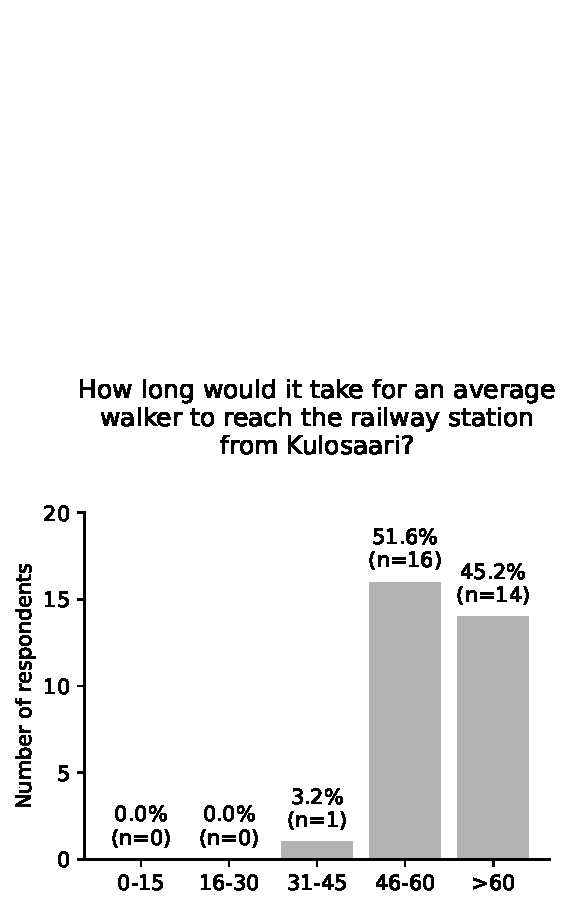
\includegraphics[width=\textwidth]{visual/figures/survey/0.pdf}
		\caption{Question 1}
		\label{fig:q 1}
	\end{subfigure}%
	\hfill
	\begin{subfigure}[b]{0.5\textwidth}
		\centering
		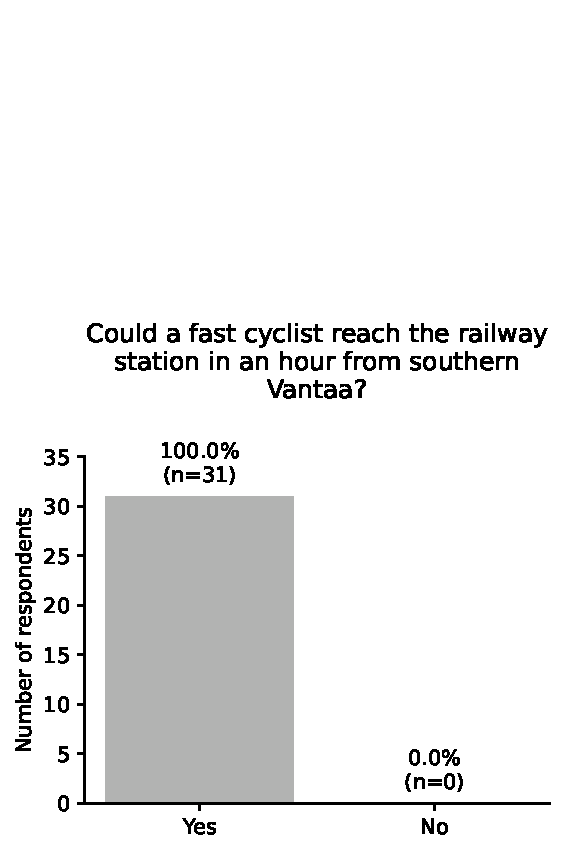
\includegraphics[width=\textwidth]{visual/figures/survey/1.pdf}
		\caption{Question 2}
		\label{fig:q 2}
	\end{subfigure}%
	\caption{Questions 1 and 2}
	\label{fig:q 1 and 2}
\end{figure}

\begin{figure}[H]
	\centering
	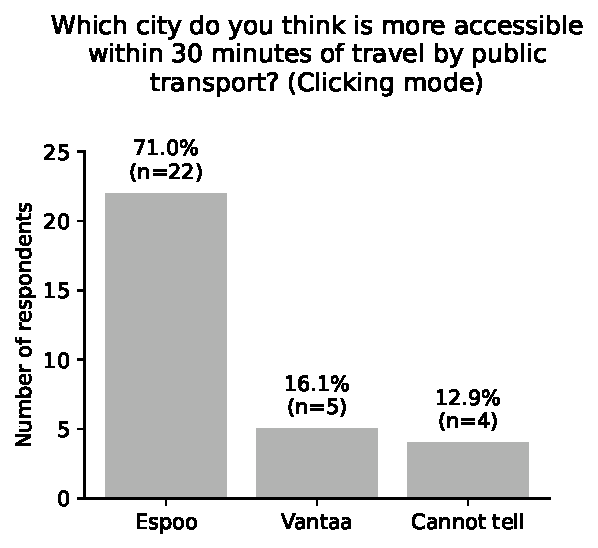
\includegraphics[width=0.5\textwidth]{visual/figures/survey/2.pdf}
	\caption{Question 3}
	\label{fig:q 3}
\end{figure}

\begin{figure}[H]
	\centering
	\begin{subfigure}[b]{0.5\textwidth}
		\centering
		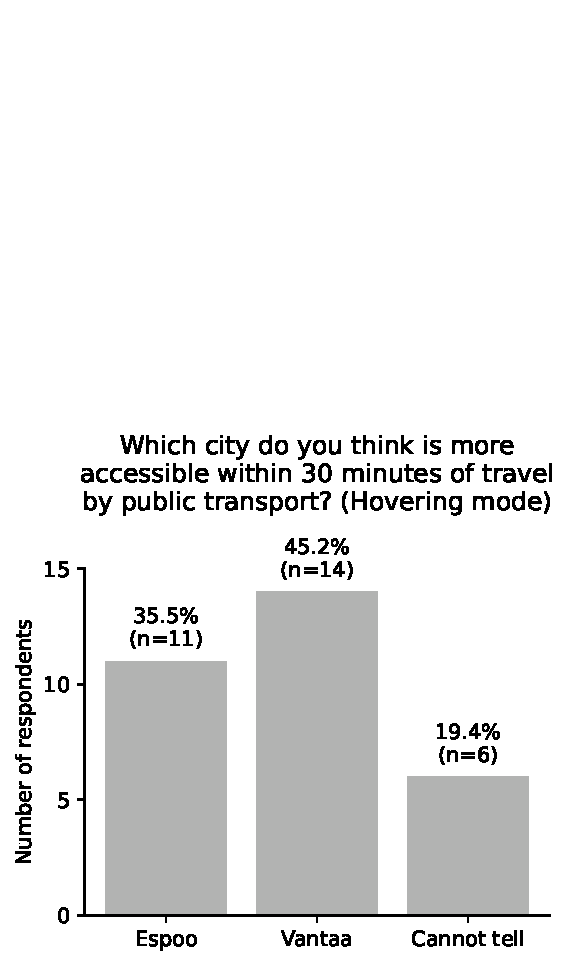
\includegraphics[width=\textwidth]{visual/figures/survey/3.pdf}
		\caption{Question 4}
		\label{fig:q 4}
	\end{subfigure}%
	\hfill
	\begin{subfigure}[b]{0.5\textwidth}
		\centering
		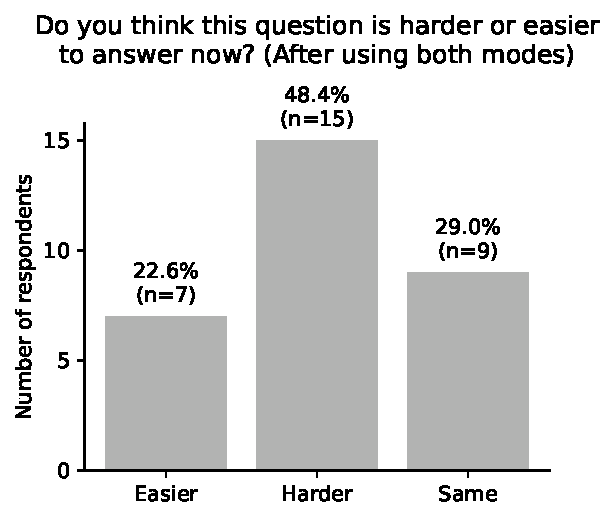
\includegraphics[width=\textwidth]{visual/figures/survey/4.pdf}
		\caption{Question 5}
		\label{fig:q 5}
	\end{subfigure}%
	\caption{Questions 4 and 5}
	\label{fig:q 4 and 5}
\end{figure}

\begin{figure}[H]
	\centering
	\begin{subfigure}[b]{0.5\textwidth}
		\centering
		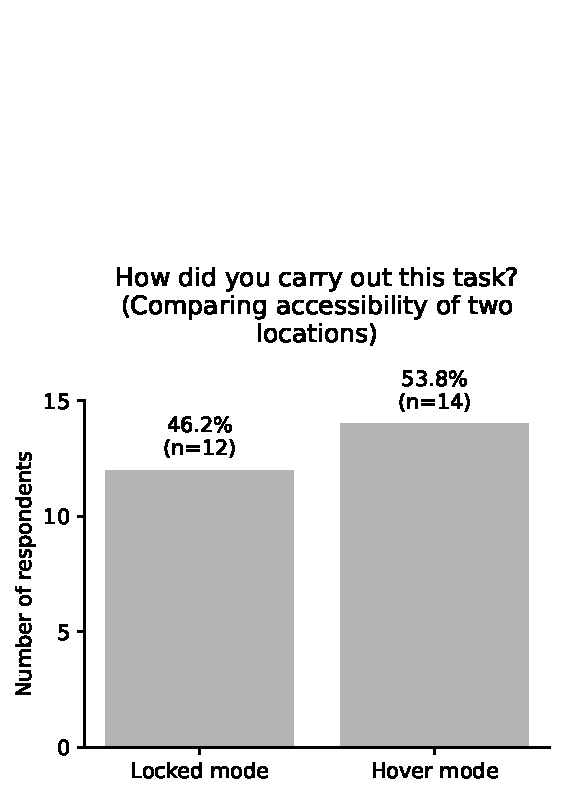
\includegraphics[width=\textwidth]{visual/figures/survey/5.pdf}
		\caption{Question 6}
		\label{fig:q 6}
	\end{subfigure}%
	\hfill
	\begin{subfigure}[b]{0.5\textwidth}
		\centering
		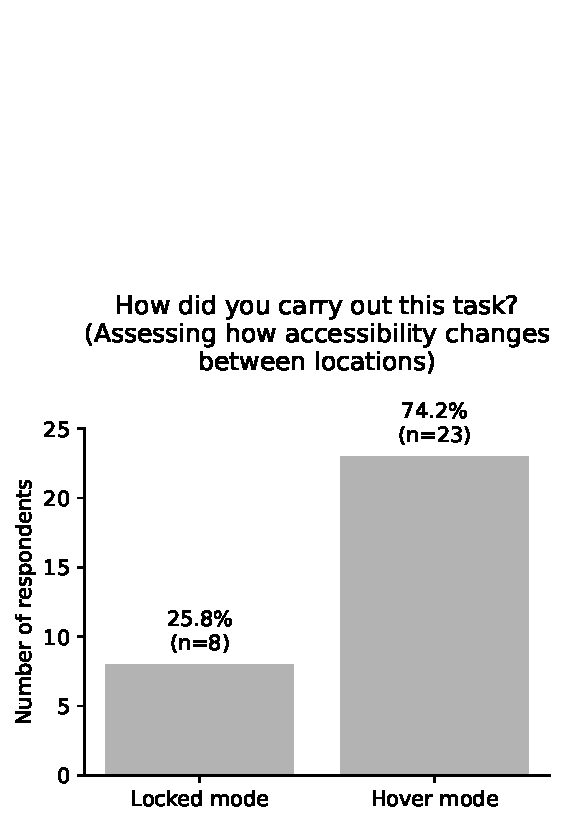
\includegraphics[width=\textwidth]{visual/figures/survey/6.pdf}
		\caption{Question 7}
		\label{fig:q 7}
	\end{subfigure}%
	\caption{Questions 6 and 7}
	\label{fig:q 6 and 7}
\end{figure}

\begin{figure}[H]
	\centering
	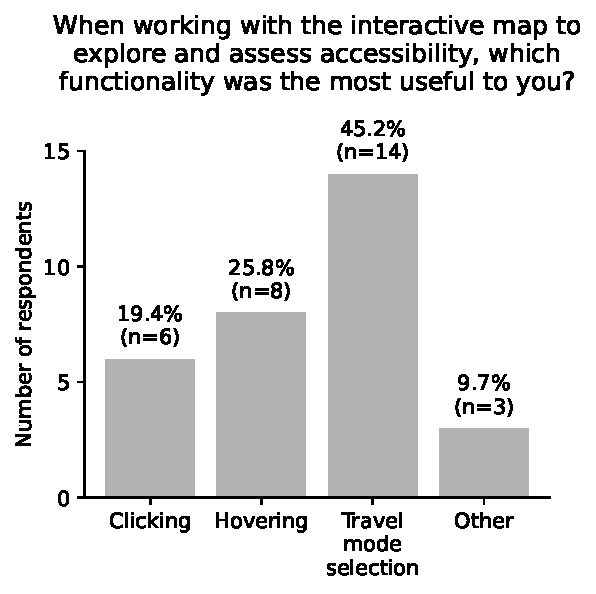
\includegraphics[width=0.5\textwidth]{visual/figures/survey/7.pdf}
	\caption{Question 8}
	\label{fig:q 8}
\end{figure}

\begin{figure}[H]
	\centering
	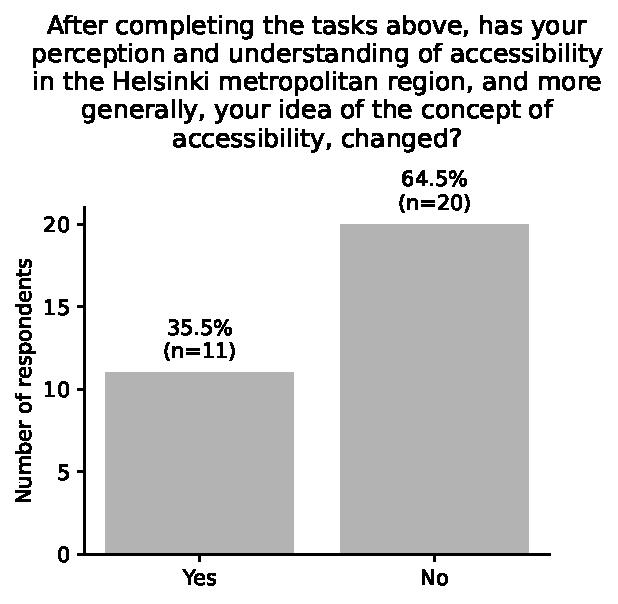
\includegraphics[width=0.5\textwidth]{visual/figures/survey/8.pdf}
	\caption{Question 9}
	\label{fig:q 9}
\end{figure}

\begin{figure}[H]
	\centering
	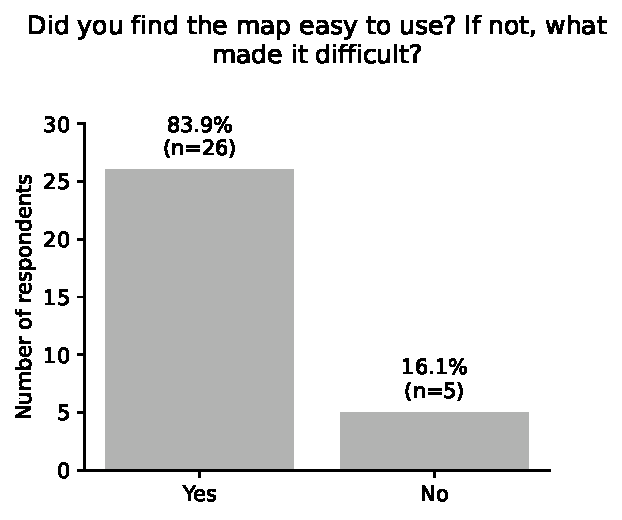
\includegraphics[width=0.5\textwidth]{visual/figures/survey/9.pdf}
	\caption{Question 10}
	\label{fig:q 10}
\end{figure}

\begin{figure}[H]
	\centering
	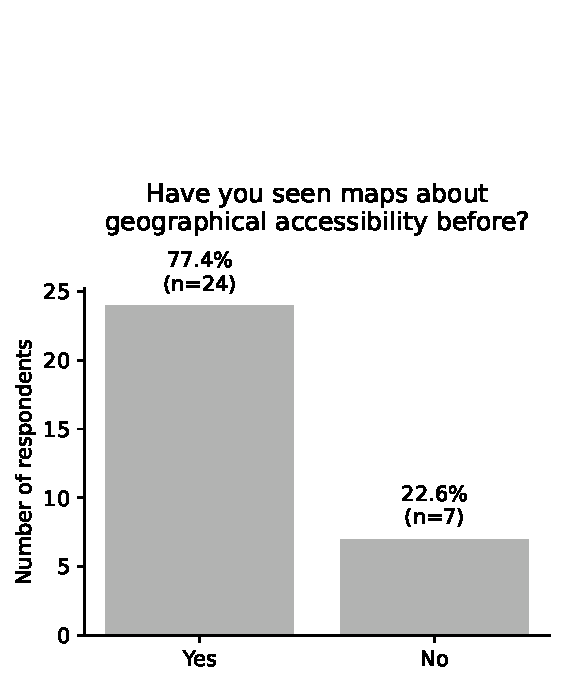
\includegraphics[width=0.5\textwidth]{visual/figures/survey/10.pdf}
	\caption{Question 11}
	\label{fig:q 11}
\end{figure}

\begin{figure}[H]
	\centering
	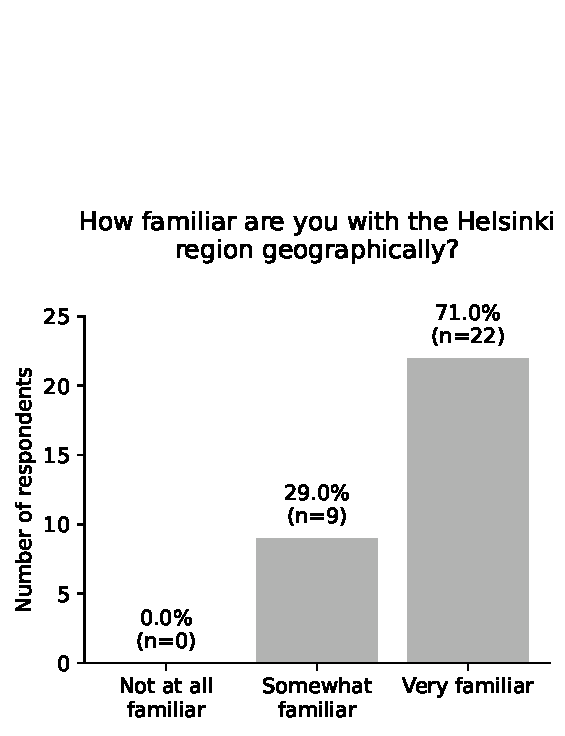
\includegraphics[width=0.5\textwidth]{visual/figures/survey/11.pdf}
	\caption{Question 12}
	\label{fig:q 12}
\end{figure}

\begin{figure}[H]
	\centering
	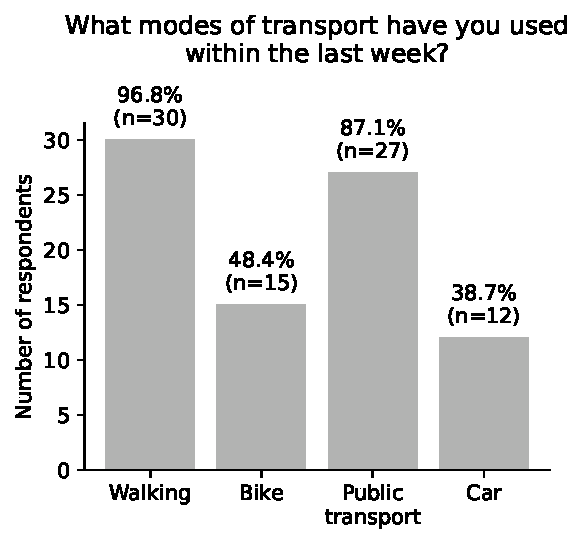
\includegraphics[width=0.5\textwidth]{visual/figures/survey/modes.pdf}
	\caption{Question 13}
	\label{fig:q 13}
\end{figure}

\begin{figure}[H]
	\centering
	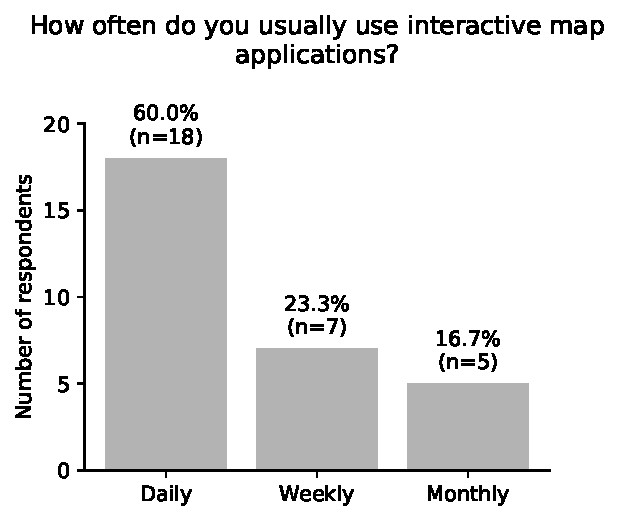
\includegraphics[width=0.5\textwidth]{visual/figures/survey/12.pdf}
	\caption{Question 14}
	\label{fig:q 14}
\end{figure}

\begin{figure}[H]
	\centering
	\begin{subfigure}[b]{0.5\textwidth}
		\centering
		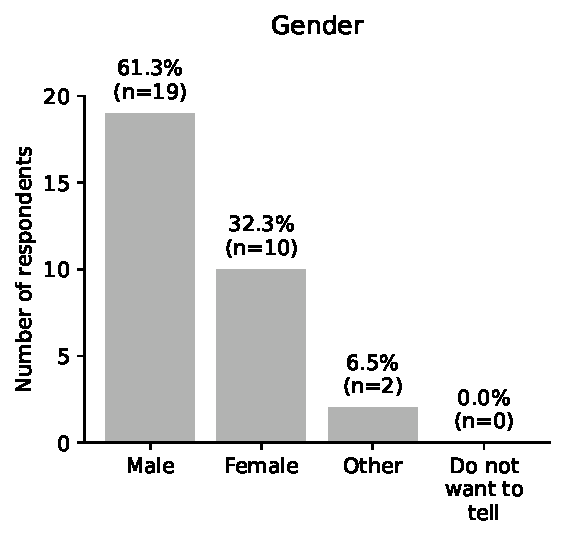
\includegraphics[width=\textwidth]{visual/figures/survey/13.pdf}
		\caption{Question 15}
		\label{fig:q 15}
	\end{subfigure}%
	\hfill
	\begin{subfigure}[b]{0.5\textwidth}
		\centering
		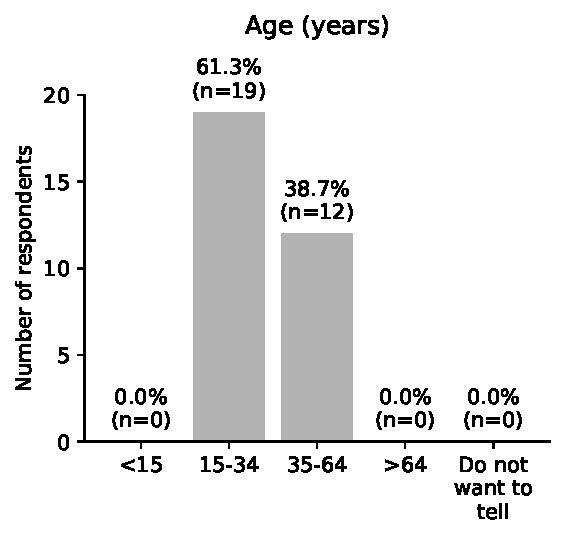
\includegraphics[width=\textwidth]{visual/figures/survey/14.pdf}
		\caption{Question 16}
		\label{fig:q 16}
	\end{subfigure}%
	\caption{Questions 15 and 16}
	\label{fig:q 15 and 16}
\end{figure}
